\documentclass[11pt,a4paper]{article}
\usepackage[margin=2.3cm,headheight=14pt]{geometry}
\usepackage{lmodern}
\usepackage[T1]{fontenc}
\usepackage{amsmath,amssymb,bm}
\usepackage{booktabs,array,tabularx}
\usepackage{graphicx}
\usepackage[dvipsnames]{xcolor}
\usepackage{tikz}
\usetikzlibrary{arrows.meta,calc,patterns,positioning,shapes.geometric}
\usepackage[skins,breakable]{tcolorbox}
\usepackage{caption}
\usepackage{float}
\usepackage{fancyhdr}
\usepackage{enumitem}
\usepackage{listings}
\usepackage{microtype}
\usepackage[colorlinks=true,linkcolor=NavyBlue,citecolor=NavyBlue,urlcolor=NavyBlue]{hyperref}

\captionsetup{font=small,labelfont=bf}
\setlength{\parskip}{0.45em}
\setlength{\parindent}{0pt}
\numberwithin{equation}{section}

\definecolor{note}{HTML}{1F4E79}
\definecolor{code}{HTML}{2A7F62}
\definecolor{warn}{HTML}{C0392B}
\definecolor{keybg}{HTML}{F3F7FB}

\lstset{basicstyle=\ttfamily\small,columns=fullflexible,keepspaces=true,
  backgroundcolor=\color{black!3},frame=leftline,rulecolor=\color{code},framerule=2pt,
  xleftmargin=8pt,framexleftmargin=6pt,aboveskip=6pt,belowskip=6pt,
  commentstyle=\color{black!55},keywordstyle=\color{note}\bfseries,language=Python,
  showstringspaces=false,breaklines=true,breakatwhitespace=true}
\newcommand{\code}[1]{\texttt{\detokenize{#1}}}
\newcommand{\opt}[1]{\texttt{-{}-#1}}

\newtcolorbox{incode}[1][]{enhanced,breakable,colback=code!5,colframe=code,
  boxrule=0pt,leftrule=3pt,arc=0pt,left=6pt,right=6pt,top=4pt,bottom=4pt,
  title={\textbf{In the code}#1},coltitle=code,colbacktitle=code!5,
  attach title to upper={\ \ },fonttitle=\small}
\newtcolorbox{idea}[1][Key idea]{enhanced,breakable,colback=note!4,colframe=note,
  boxrule=0pt,leftrule=3pt,arc=0pt,left=6pt,right=6pt,top=4pt,bottom=4pt,
  title={\textbf{#1}},coltitle=note,colbacktitle=note!4,
  attach title to upper={\ \ },fonttitle=\small}
\newtcolorbox{pitfall}[1][Watch out]{enhanced,breakable,colback=warn!4,colframe=warn,
  boxrule=0pt,leftrule=3pt,arc=0pt,left=6pt,right=6pt,top=4pt,bottom=4pt,
  title={\textbf{#1}},coltitle=warn,colbacktitle=warn!4,
  attach title to upper={\ \ },fonttitle=\small}

\pagestyle{fancy}
\fancyhf{}
\fancyhead[L]{\small Eccentric-cavity soft bending actuator}
\fancyhead[R]{\small Nonlinear 3-D FEA: a beginner's handbook}
\fancyfoot[C]{\small\thepage}
\renewcommand{\headrulewidth}{0.4pt}

\newcommand{\F}{\mathbf{F}}
\newcommand{\X}{\mathbf{X}}
\newcommand{\x}{\mathbf{x}}
\newcommand{\uu}{\mathbf{u}}
\newcommand{\K}{\mathbf{K}}
\newcommand{\R}{\mathbf{R}}
\newcommand{\Ib}{\bar I_1}

\begin{document}

%======================================================================
\begin{titlepage}
\centering
\vspace*{2.4cm}
{\large B.Tech Project\par}
\vspace{0.6cm}
{\LARGE\bfseries How our nonlinear 3-D FEA works\par}
\vspace{0.4cm}
{\Large A beginner's handbook to \texttt{actuator\_fea.py}\par}
\vspace{1.4cm}

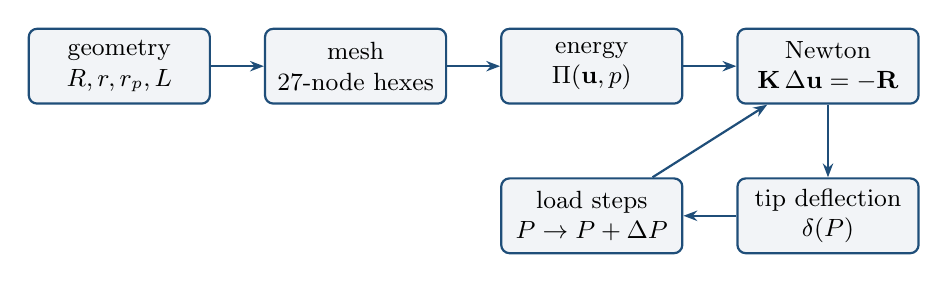
\begin{tikzpicture}[scale=1.0,
  box/.style={draw=note,thick,rounded corners=3pt,fill=note!6,minimum width=2.3cm,minimum height=0.95cm,align=center,font=\small},
  arr/.style={-{Stealth[length=5pt]},thick,note}]
  \node[box] (g) at (0,0) {geometry\\$R,r,r_p,L$};
  \node[box] (m) at (3,0) {mesh\\27-node hexes};
  \node[box] (e) at (6,0) {energy\\$\Pi(\uu,p)$};
  \node[box] (n) at (9,0) {Newton\\$\K\,\Delta\uu=-\R$};
  \node[box] (o) at (9,-1.9) {tip deflection\\$\delta(P)$};
  \node[box] (s) at (6,-1.9) {load steps\\$P\to P+\Delta P$};
  \draw[arr] (g)--(m); \draw[arr] (m)--(e); \draw[arr] (e)--(n);
  \draw[arr] (n)--(o); \draw[arr] (s)--(n); \draw[arr] (o.west)--++(-0.4,0) |- (s.east);
\end{tikzpicture}

\vspace{1.4cm}
{\large Rudranarayan Pradhan\par}
\vspace{0.3cm}
{\normalsize October 2026\par}
\vfill
\begin{minipage}{0.86\textwidth}
\small\textbf{What this is.}
A step-by-step explanation of the finite-element code we wrote to predict how far
the eccentric-cavity actuator bends under pressure. It assumes only first-year
mechanics and calculus. Each section explains one idea in plain terms, gives the
equation, and then points to the exact lines of \texttt{actuator\_fea.py} that
implement it, so the handbook can be read side by side with the code. Line numbers
refer to the version of the code in the project folder on 8 October 2026.
\end{minipage}
\vspace{0.6cm}
\end{titlepage}

\tableofcontents
\newpage

%======================================================================
\section{The big picture}

\paragraph{The question.}
Our actuator is a silicone cylinder (radius $R=10$\,mm, length $L=100$\,mm) with a
cylindrical cavity (radius $r=4$\,mm) placed $r_p=3$\,mm off the centre. When the
cavity is pressurised, the thin side of the wall stretches more than the thick side
and the cylinder curls towards the thick side. We want the tip deflection $\delta$
as a function of the pressure $P$.

\paragraph{Why hand formulas are not enough.}
The beam formulas in the derivation report assume small strains and a linear
material. In our actuator the silicone stretches by up to 2.5 times, the material
gets stiffer in a nonlinear way, and the pressure keeps pushing perpendicular to the
wall even as the wall moves. All three effects are \emph{nonlinear}. The finite
element method (FEM, or FEA for finite element analysis) handles them by solving
the full 3-D equations of large-deformation elasticity numerically.

\paragraph{Why we wrote our own code.}
No structural FE package (ANSYS, Abaqus, COMSOL) was installed. Instead we wrote a
compact solver in Python (\texttt{actuator\_fea.py}, about 530 lines) on top of
\texttt{numpy}, \texttt{scipy} and \texttt{jax}. Writing it ourselves has one big
advantage for a project: every modelling choice is visible and can be checked.

\paragraph{The pipeline.}
Figure~\ref{fig:pipeline} shows what happens when you run the code. Each box is a
section of this handbook.

\begin{figure}[H]
\centering
\begin{tikzpicture}[
  box/.style={draw=note,thick,rounded corners=3pt,fill=note!6,text width=3.4cm,minimum height=1.0cm,align=center,font=\small},
  arr/.style={-{Stealth[length=5pt]},thick,note}]
  \node[box] (a) at (0,0) {\textbf{Mesh} (\S\ref{sec:mesh})\\split the half actuator into 588 curved bricks};
  \node[box] (b) at (4.6,0) {\textbf{Element energy} (\S\ref{sec:kin}--\ref{sec:element})\\strain energy of the silicone in each brick};
  \node[box] (c) at (9.2,0) {\textbf{Loads and supports} (\S\ref{sec:bc}--\ref{sec:pressure})\\clamp, symmetry, sleeve, pressure $-PV$};
  \node[box] (d) at (9.2,-2.3) {\textbf{Equilibrium} (\S\ref{sec:equil})\\residual $\R(\uu)=\mathbf{0}$};
  \node[box] (e) at (4.6,-2.3) {\textbf{Newton} (\S\ref{sec:newton})\\tangent by autodiff, sparse solve};
  \node[box] (f) at (0,-2.3) {\textbf{Load stepping} (\S\ref{sec:steps})\\pressure, then volume control};
  \node[box] (g) at (4.6,-4.6) {\textbf{Post-processing} (\S\ref{sec:post})\\$\theta$, $\delta$, stretch, wall thickness};
  \draw[arr] (a)--(b); \draw[arr] (b)--(c); \draw[arr] (c)--(d); \draw[arr] (d)--(e);
  \draw[arr] (f)--(e); \draw[arr] (e) to[bend left=25] node[below,font=\scriptsize]{converged} (f);
  \draw[arr] (f) |- (g);
\end{tikzpicture}
\caption{What \texttt{actuator\_fea.py} does, in order.}
\label{fig:pipeline}
\end{figure}

\begin{idea}
FEA turns one impossible problem (find the exact deformed shape of a 3-D rubber
body) into a very large but ordinary one (find about 18\,000 numbers, the
displacements of the mesh nodes, that make the forces balance).
\end{idea}

%======================================================================
\section{FEA in one dimension: the whole method on a bar}
\label{sec:1d}

Everything the 3-D code does already appears in a 1-D bar, so we start there.

\paragraph{Step 1: cut the body into elements.}
Take a bar of length $3a$, axial stiffness $EA$, clamped at the left and pulled by a
force $F$ at the right. Cut it into three \emph{elements} joined at four
\emph{nodes} (Figure~\ref{fig:bar}).

\begin{figure}[H]
\centering
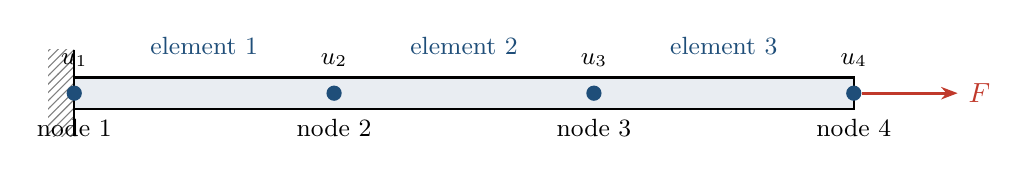
\begin{tikzpicture}[scale=1.1]
  \fill[pattern=north east lines,pattern color=black!50] (-0.3,-0.5) rectangle (0,0.5);
  \draw[thick] (0,-0.5)--(0,0.5);
  \fill[note!10] (0,-0.18) rectangle (9,0.18);
  \draw[thick] (0,-0.18) rectangle (9,0.18);
  \foreach \i/\xx in {1/0,2/3,3/6,4/9} {
    \fill[note] (\xx,0) circle (2.5pt);
    \node[below=6pt,font=\small] at (\xx,0) {node \i};
    \node[above=6pt,font=\small] at (\xx,0) {$u_\i$};
  }
  \foreach \e/\xx in {1/1.5,2/4.5,3/7.5} \node[font=\small,note] at (\xx,0.55) {element \e};
  \draw[-{Stealth[length=6pt]},very thick,warn] (9.1,0)--(10.2,0) node[right]{$F$};
\end{tikzpicture}
\caption{A bar cut into three two-node elements.}
\label{fig:bar}
\end{figure}

\paragraph{Step 2: guess a shape inside each element.}
Inside an element we do not know the displacement $u(X)$, so we \emph{interpolate}
it from the node values with \emph{shape functions}. For a two-node element of length
$a$ the simplest choice is a straight line:
\begin{equation}
u(\xi) = N_1(\xi)\,u_i + N_2(\xi)\,u_j,\qquad N_1=\tfrac12(1-\xi),\quad N_2=\tfrac12(1+\xi),
\end{equation}
where $\xi\in[-1,1]$ is a local coordinate along the element. Our 3-D code uses
quadratic instead of linear shape functions, in three directions (\S\ref{sec:element}),
but the idea is identical.

\paragraph{Step 3: write the energy.}
The strain in an element is $\varepsilon=(u_j-u_i)/a$ and its stored energy is
$\tfrac12 EA\,a\,\varepsilon^2=\tfrac12 k(u_j-u_i)^2$ with $k=EA/a$. The total
potential energy is the stored energy minus the work done by the load:
\begin{equation}
\Pi(\uu)=\tfrac12 k(u_2-u_1)^2+\tfrac12 k(u_3-u_2)^2+\tfrac12 k(u_4-u_3)^2-F\,u_4 .
\end{equation}

\paragraph{Step 4: equilibrium means the energy is stationary.}
The bar settles where $\Pi$ is a minimum, $\partial\Pi/\partial u_n=0$ for every free
node. Writing this out gives the familiar matrix equation $\K\uu=\mathbf{f}$:
\begin{equation}
k\begin{bmatrix}2&-1&0\\-1&2&-1\\0&-1&1\end{bmatrix}
\begin{bmatrix}u_2\\u_3\\u_4\end{bmatrix}=\begin{bmatrix}0\\0\\F\end{bmatrix}
\quad\Longrightarrow\quad u_2=\frac{F}{k},\;u_3=\frac{2F}{k},\;u_4=\frac{3F}{k}=\frac{F\cdot 3a}{EA}.
\end{equation}
$u_1=0$ is the clamp: its row and column are simply removed. Each element contributes
a small $2\times2$ block $k\left[\begin{smallmatrix}1&-1\\-1&1\end{smallmatrix}\right]$
to the big matrix; adding these blocks into the right rows and columns is called
\emph{assembly}.

\paragraph{Step 5: what changes when the problem is nonlinear.}
For a rubber bar the force is no longer proportional to the stretch. For an
incompressible neo-Hookean bar the nominal stress is $s=\mu(\lambda-\lambda^{-2})$,
so to find the stretch at which $s=0.5\mu$ we must solve
$R(\lambda)=\lambda-\lambda^{-2}-0.5=0$. We cannot rearrange it, so we use
\emph{Newton's method}: linearise, solve, repeat,
\begin{equation}
\lambda_{k+1}=\lambda_k-\frac{R(\lambda_k)}{R'(\lambda_k)},\qquad R'(\lambda)=1+2\lambda^{-3}.
\end{equation}

\begin{center}
\begin{tabular}{ccc}
\toprule
iteration $k$ & $\lambda_k$ & residual $R(\lambda_k)$\\
\midrule
0 & 1.000000 & $-5.0\times10^{-1}$\\
1 & 1.166667 & $-6.8\times10^{-2}$\\
2 & 1.196774 & $-1.4\times10^{-3}$\\
3 & 1.197429 & $-6.3\times10^{-7}$\\
4 & 1.197429 & $-1.2\times10^{-13}$\\
\bottomrule
\end{tabular}
\end{center}

The number of correct digits roughly doubles every iteration: this is
\emph{quadratic convergence}, and it is exactly what we see in the 3-D runs, where
each pressure step converges in 3 to 6 iterations.

\begin{idea}[The whole method in four words]
\textbf{Interpolate, integrate, assemble, iterate.} The 3-D code does these same
steps with $27$-node bricks instead of 2-node bars, a rubber energy instead of
$\tfrac12k\varepsilon^2$, and about 18\,000 unknowns instead of three.
\end{idea}

%======================================================================
\section{Describing large deformation}
\label{sec:kin}

\paragraph{Reference and current positions.}
Every material point has a position $\X$ in the undeformed (\emph{reference}) body
and a position $\x=\X+\uu$ after deformation, where $\uu$ is the displacement. All our
unknowns are nodal displacements.

\paragraph{The deformation gradient.}
How a tiny fibre $d\X$ is stretched and rotated is described by the $3\times3$ matrix
\begin{equation}
\F=\frac{\partial\x}{\partial\X},\qquad d\x=\F\,d\X .
\end{equation}
Two quantities built from $\F$ matter for rubber:
\begin{itemize}[nosep]
\item the \textbf{volume ratio} $J=\det\F$ ($J=1$ means no volume change);
\item the \textbf{shape-change invariant}
$\Ib=J^{-2/3}\,\mathrm{tr}(\F^{\mathsf T}\F)=J^{-2/3}\sum_{ij}F_{ij}^2$, which is $3$
in the undeformed state and grows as the material is distorted.
\end{itemize}
$\Ib$ ignores volume change (the factor $J^{-2/3}$ removes it), so it separates
``changing shape'' from ``changing volume''. This split is what lets us treat
incompressibility separately (\S\ref{sec:locking}).

\paragraph{Stretch.}
The principal stretches $\lambda_1\ge\lambda_2\ge\lambda_3$ are the square roots of the
eigenvalues of $\mathbf{C}=\F^{\mathsf T}\F$. The largest one, $\lambda_1$, is what
we plot as ``peak principal stretch''.

\begin{incode}
\code{_elem_pi} (line 184) computes \code{F} at all 27 Gauss points from the current
nodal positions, \code{J = _det3(F)} (line 178), and
\code{d = J**(-2/3) * sum(F*F) - 3}, which is $\Ib-3$. \code{FEModel.stretch} (line
303) computes $\lambda_1$ per element with \code{np.linalg.eigvalsh}.
\end{incode}

%======================================================================
\section{The material: hyperelastic silicone}
\label{sec:material}

Rubber-like materials are \emph{hyperelastic}: all their behaviour comes from a
\emph{strain-energy density} $W$, the energy stored per unit reference volume. We
use the Yeoh model:
\begin{equation}
W_{\text{iso}}=C_{10}(\Ib-3)+C_{20}(\Ib-3)^2+C_{30}(\Ib-3)^3 .
\label{eq:yeoh}
\end{equation}
With $C_{20}=C_{30}=0$ this is the \textbf{neo-Hookean} model, which we use for the
placeholder silicone. The constants link to the familiar small-strain moduli by
\begin{equation}
\mu=2C_{10}\ \ (\text{shear modulus}),\qquad E=3\mu=6C_{10}\ \ (\text{incompressible}).
\end{equation}
For $E=0.6$\,MPa this gives $C_{10}=0.1$\,MPa and $\mu=0.2$\,MPa. The higher Yeoh
terms make the silicone stiffen at large stretch; their values must come from a
tensile test of the real silicone (a task in the project timeline).

\begin{incode}
\code{Material} in \texttt{actuator\_model.py} stores $(C_{10},C_{20},C_{30})$;
\code{Material.from_E(E)} sets $C_{10}=E/6$. In \code{_elem_pi} the three Yeoh terms are
\code{c[0]*d + c[1]*d**2 + c[2]*d**3}. The command-line flag \opt{yeoh C10 C20 C30}
replaces the neo-Hookean default.
\end{incode}

%======================================================================
\section{Nearly incompressible rubber: locking and the mixed element}
\label{sec:locking}

\paragraph{The problem.}
Silicone hardly changes volume: its Poisson's ratio is almost $0.5$. We model this
with a large bulk modulus $\kappa$,
\begin{equation}
\kappa=\frac{2\mu(1+\nu)}{3(1-2\nu)},\qquad \nu=0.4995\ \Rightarrow\ \kappa\approx1000\,\mu .
\end{equation}
If we simply added a stiff volume penalty $\tfrac12\kappa(J-1)^2$ to $W$, the
elements would \emph{lock}: with only a few displacement modes per element, keeping
$J\approx1$ at every Gauss point is so restrictive that the mesh becomes far too
stiff and the predicted bending far too small. Locking is the classic trap of
rubber FEA.

\paragraph{The fix: a separate pressure field.}
We add a second unknown, an internal pressure $p$, and use the \emph{mixed} energy
\begin{equation}
W=W_{\text{iso}}(\Ib)+p\,(J-1)-\frac{p^2}{2\kappa}.
\label{eq:mixed}
\end{equation}
Making this stationary with respect to $p$ gives $J-1=p/\kappa$: the volume
constraint is now enforced through $p$ rather than through the displacements. Inside
each element $p$ is linear in the local coordinates,
\begin{equation}
p(\xi,\eta,\zeta)=p_0+p_1\xi+p_2\eta+p_3\zeta ,
\end{equation}
so it has only four coefficients and is allowed to jump between elements. This is
the well-known \textbf{Q2/P1} element (quadratic displacement, linear discontinuous
pressure), which does not lock.

\paragraph{Static condensation: getting rid of $p$.}
Because $p$ belongs to one element only, it can be eliminated element by element
before assembly. Linearising one element gives the block system
\begin{equation}
\begin{bmatrix}\K_{uu}&\K_{up}\\ \K_{pu}&\K_{pp}\end{bmatrix}
\begin{bmatrix}\Delta\uu\\ \Delta\mathbf{p}\end{bmatrix}
=-\begin{bmatrix}\mathbf{r}_u\\ \mathbf{r}_p\end{bmatrix},
\qquad \K_{pp}=-\frac{1}{\kappa}\mathbf{M},\quad \mathbf{M}=\int\bm\psi\bm\psi^{\mathsf T}dV ,
\end{equation}
where $\bm\psi=(1,\xi,\eta,\zeta)$ and $\mathbf{M}$ is the small ``pressure mass
matrix''. With $\mathbf{A}=-\K_{pp}^{-1}=\kappa\mathbf{M}^{-1}$ the second row gives
\begin{equation}
\Delta\mathbf{p}=\mathbf{A}\,(\mathbf{r}_p+\K_{pu}\Delta\uu),
\end{equation}
and substituting into the first row leaves a displacement-only system,
\begin{equation}
\big(\K_{uu}+\K_{up}\mathbf{A}\K_{pu}\big)\Delta\uu=-\big(\mathbf{r}_u+\K_{up}\mathbf{A}\,\mathbf{r}_p\big).
\label{eq:condense}
\end{equation}
The global matrix therefore has only displacement unknowns, and the pressures are
recovered afterwards from the formula for $\Delta\mathbf{p}$.

\begin{incode}
\code{FEModel.__init__}: \code{self.kappa} (line 253) and \code{self.A} (line 261).
\code{PSI} (line 59) holds $(1,\xi,\eta,\zeta)$ at the Gauss points.
In \code{FEModel.solve}: the condensed tangent \code{H_uu + KA @ Kup.T} (line 334),
the extra residual \code{Rc = KA @ rp} (line 340), and the pressure update \code{dp}
(line 351).
\end{incode}

%======================================================================
\section{The 27-node element and Gauss integration}
\label{sec:element}

\paragraph{Quadratic shape functions.}
In one direction we use three nodes at $\xi=-1,0,1$ and the quadratic Lagrange
functions
\begin{equation}
N_{-1}=\tfrac12\xi(\xi-1),\qquad N_0=1-\xi^2,\qquad N_{+1}=\tfrac12\xi(\xi+1).
\end{equation}
Each equals 1 at its own node and 0 at the other two. Multiplying one function from
each of the three directions gives $3\times3\times3=27$ shape functions for a brick
with 27 nodes: 8 corners, 12 edge midpoints, 6 face centres and 1 centre.

\paragraph{The isoparametric map.}
The same shape functions describe the element's geometry: the reference cube
$[-1,1]^3$ is mapped onto the real, curved brick by $\X(\bm\xi)=\sum_a N_a(\bm\xi)\X_a$
(Figure~\ref{fig:iso}). Because the functions are quadratic, element edges can be
curved, which lets a coarse mesh follow the circular cavity and outer surface
closely. The chain rule then gives the derivatives we need for $\F$:
\begin{equation}
\frac{\partial N_a}{\partial\X}=\frac{\partial N_a}{\partial\bm\xi}\,\mathbf{J}_0^{-1},
\qquad \mathbf{J}_0=\frac{\partial\X}{\partial\bm\xi}.
\end{equation}

\begin{figure}[H]
\centering
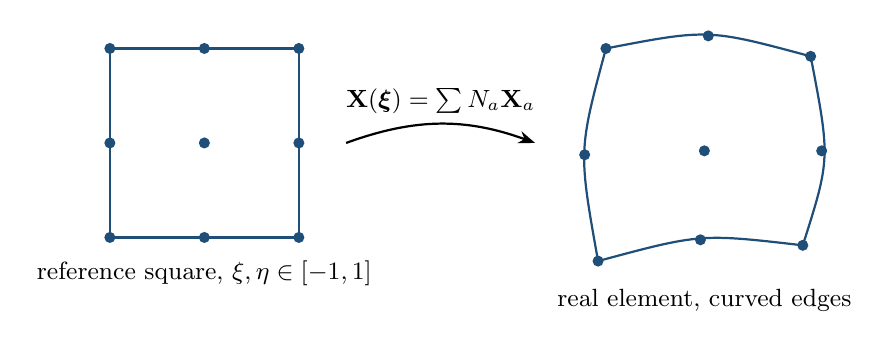
\begin{tikzpicture}[scale=1.0]
  \draw[thick,note] (0,0) rectangle (2.4,2.4);
  \foreach \i in {0,1.2,2.4} \foreach \j in {0,1.2,2.4} \fill[note] (\i,\j) circle (2pt);
  \node[font=\small] at (1.2,-0.45) {reference square, $\xi,\eta\in[-1,1]$};
  \draw[-{Stealth[length=6pt]},thick] (3.0,1.2) to[bend left=20] node[above,font=\small]{$\X(\bm\xi)=\sum N_a\X_a$} (5.4,1.2);
  \begin{scope}[shift={(6.2,-0.3)}]
    \draw[thick,note] (0,0) .. controls (1.3,0.35) .. (2.6,0.2)
      .. controls (2.95,1.3) .. (2.7,2.6)
      .. controls (1.4,2.95) .. (0.1,2.7)
      .. controls (-0.25,1.4) .. (0,0);
    \foreach \p in {(0,0),(1.3,0.27),(2.6,0.2),(2.84,1.4),(2.7,2.6),(1.4,2.86),(0.1,2.7),(-0.17,1.35),(1.35,1.4)}
      \fill[note] \p circle (2pt);
    \node[font=\small] at (1.35,-0.5) {real element, curved edges};
  \end{scope}
\end{tikzpicture}
\caption{The isoparametric idea, drawn in 2-D (a 9-node face of the 27-node brick).}
\label{fig:iso}
\end{figure}

\paragraph{Gauss integration.}
The element energy $\int W\,dV$ cannot be integrated by hand, so we evaluate $W$ at
a few special points and take a weighted sum. Three Gauss points per direction,
at $\xi=-\sqrt{0.6},\,0,\,+\sqrt{0.6}$ with weights $5/9,\,8/9,\,5/9$, integrate
polynomials up to degree five exactly. In 3-D that is $27$ points, and
\begin{equation}
\int_{\text{element}}W\,dV\approx\sum_{g=1}^{27}w_g\,\det\mathbf{J}_0(\bm\xi_g)\,W(\F_g).
\end{equation}

\begin{incode}
\code{_lagrange} (line 41) gives $N$ and $dN/d\xi$; \code{_GP}, \code{_GW} (lines 49--50) are
the Gauss points and weights; \code{_tp3} (line 54) builds the 27 tensor products;
\code{DN3} and \code{W3} (lines 57--58) are their derivatives and weights.
\code{FEModel.__init__} stores \code{dNdX} (line 258) and \code{wdV} $=w_g\det\mathbf{J}_0$
(line 259) once, since the reference mesh never changes.
\end{incode}

%======================================================================
\section{Building the actuator mesh}
\label{sec:mesh}

\paragraph{Half model.}
The actuator and its loading are symmetric about the bending plane $z=0$, so we mesh
only the half $z\ge0$ and impose symmetry on the cut (\S\ref{sec:bc}). This halves
the cost with no loss of accuracy.

\paragraph{The cross-section: rays from the cavity centre.}
The wall is meshed with rays from the cavity centre $C=(0,r_p)$ at angle $\phi$ from
the thin side. Each ray starts at the cavity (distance $r$) and ends on the outer
circle, at distance
\begin{equation}
\rho_{\text{out}}(\phi)=\sqrt{R^2-r_p^2\sin^2\phi}-r_p\cos\phi=r+t(\phi),
\end{equation}
which is exactly the wall-thickness formula $t(\phi)$ from the derivation report.
Nodes are spaced evenly along each ray. The section is then copied along $x$ to make
the 3-D wall (Figure~\ref{fig:mesh}).

\paragraph{The tip cap.}
At $x=L$ the cavity is closed by a solid cap of thickness $R/2=5$\,mm. Filling the
circular cavity area with bricks needs a small square core and a ring of elements
around it, so the cap is built from three blocks.

\paragraph{Gluing blocks together.}
The blocks are built separately and then merged: nodes that sit at the same point
are found with a $k$-d tree and given one number. Nodes are numbered along $x$, which
keeps the stiffness matrix narrow (banded) and the sparse solver fast.

\paragraph{Mesh size.}
The ``medium'' mesh used for all results has 12 elements round the half
circumference, 2 through the wall and 20 along the length, plus the cap: 588
elements, 6205 nodes and 17\,725 free displacement unknowns. Going to the fine mesh
(1664 elements) changes the tip deflection by less than 0.5\,\% (\S\ref{sec:verify}).

\begin{figure}[H]
\centering
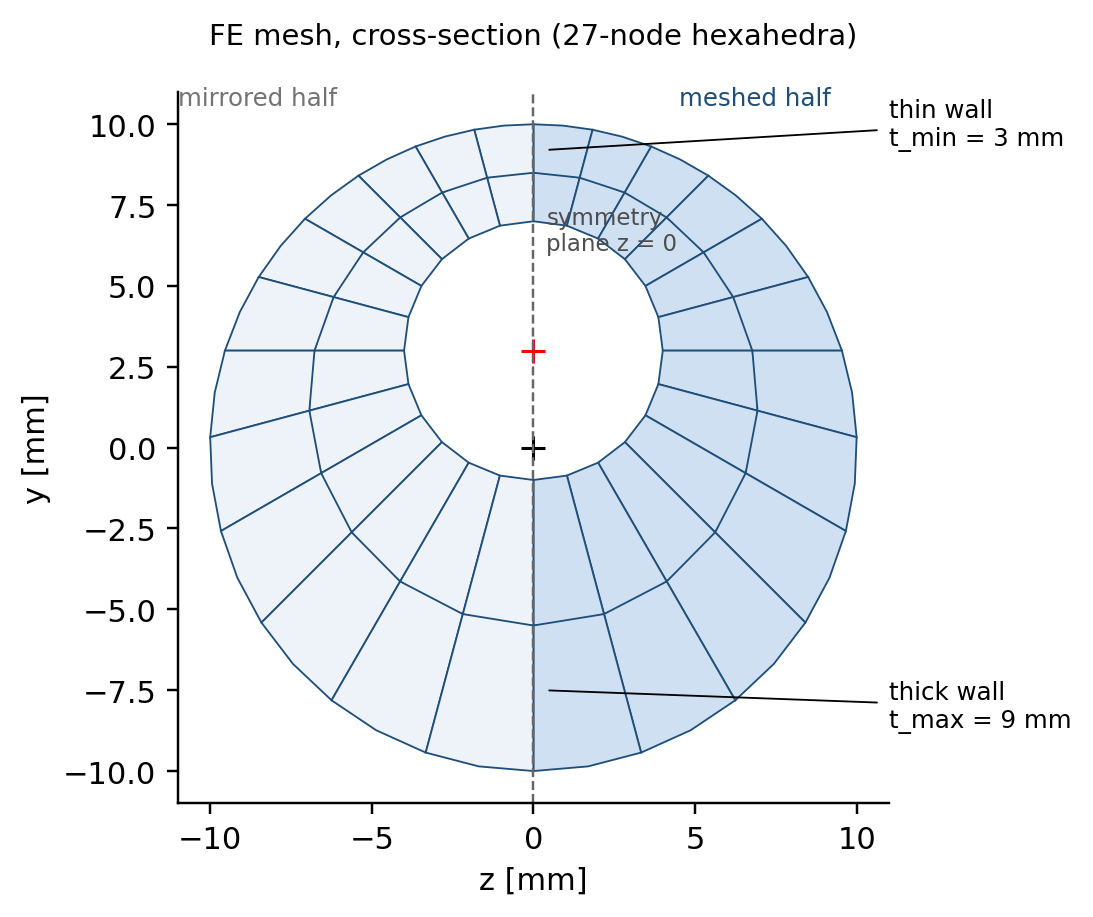
\includegraphics[width=0.62\textwidth]{figures/fe_mesh_section.png}\\[4pt]
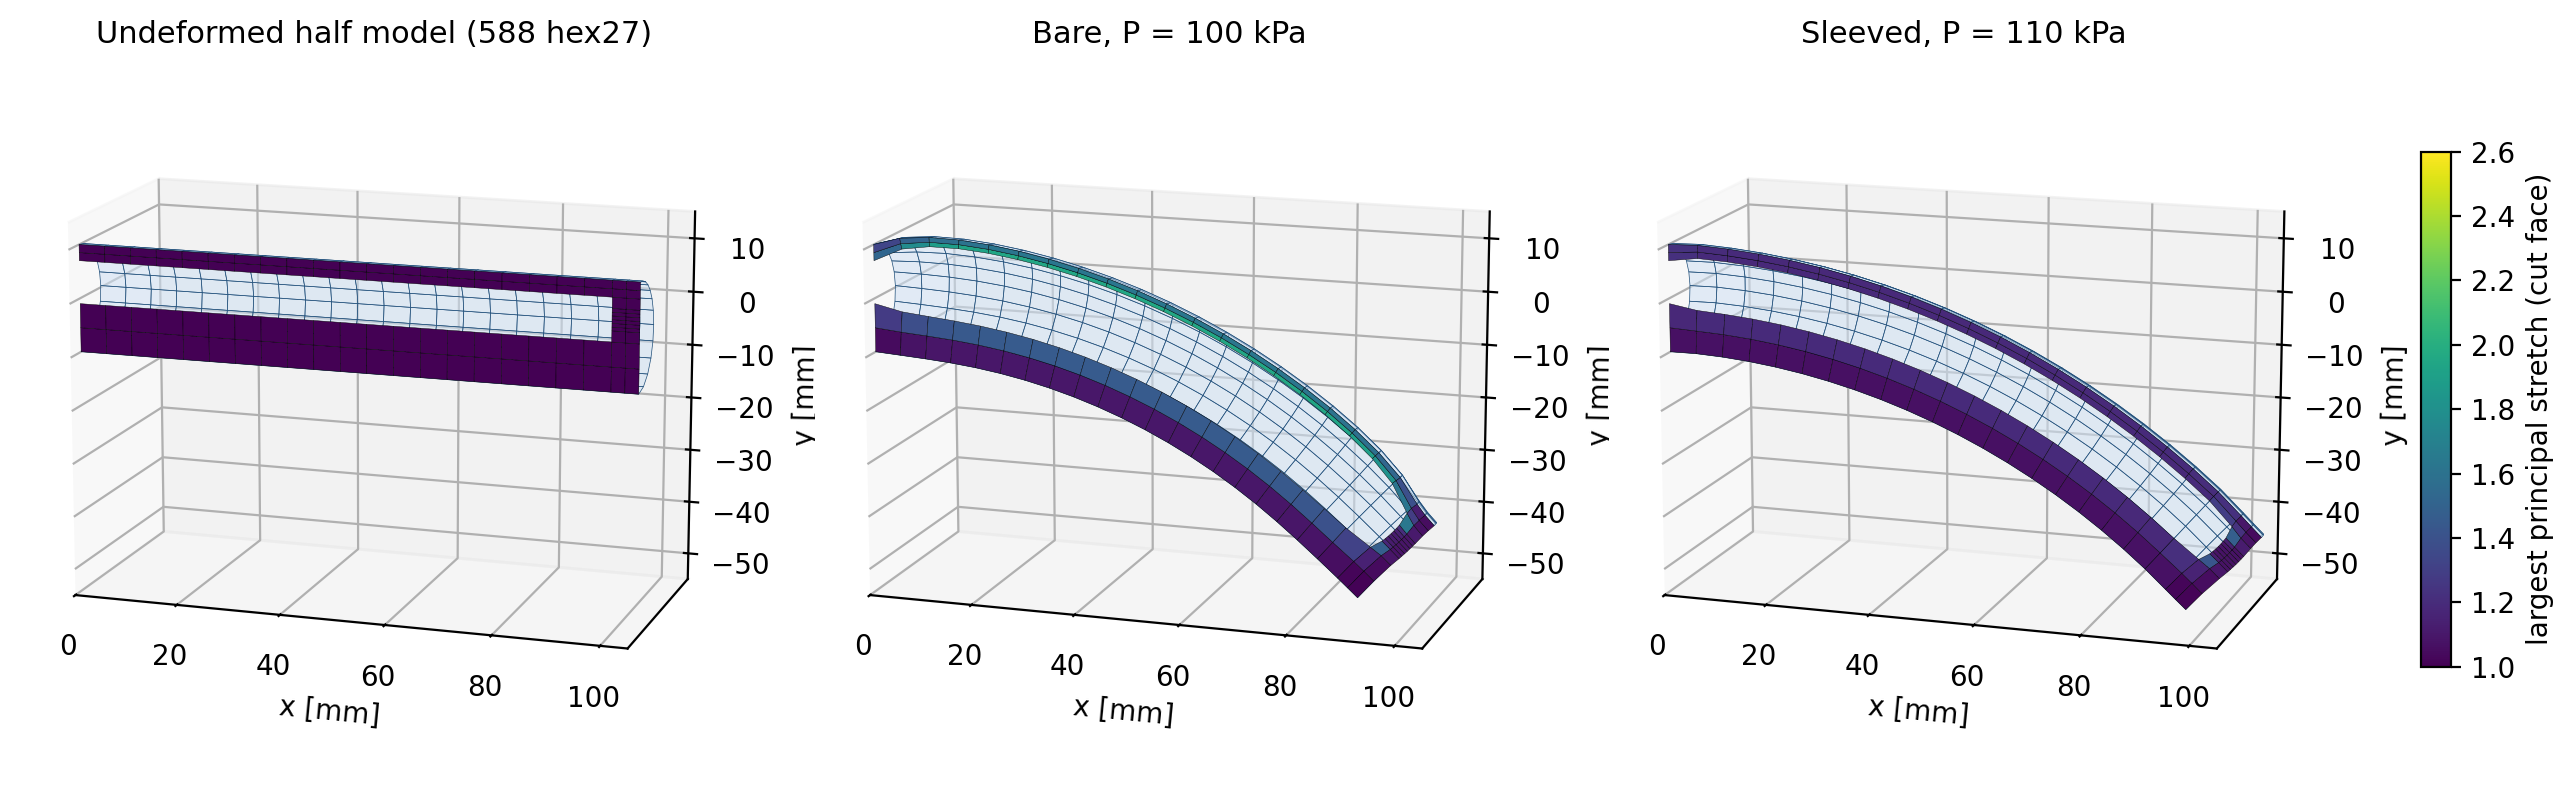
\includegraphics[width=\textwidth]{figures/fe_mesh_3d.png}
\caption{Top: the cross-section mesh, built from rays out of the cavity centre.
Bottom: the 3-D half model, undeformed and deformed.}
\label{fig:mesh}
\end{figure}

\begin{incode}
\code{MESH_PRESETS} (line 68), \code{build_mesh} (line 131): the ray formula is line 143,
the cap blocks lines 147--155, the merge line 158. \code{merge_blocks} (line 87) uses
\code{cKDTree}; \code{right_handed} (line 106) flips any element whose local axes came
out left-handed (negative Jacobian); \code{orient_faces} (line 114) makes every cavity
face normal point out of the fluid.
\end{incode}

%======================================================================
\section{Supports, symmetry and the sleeve}
\label{sec:bc}

\paragraph{Clamp.}
The base face $x=0$ is glued to a fixed mount: all three displacement components of
its nodes are zero.

\paragraph{Symmetry.}
On the cut plane $z=0$ points can move in $x$ and $y$ but not through the plane:
$u_z=0$. This is the mathematical statement that the missing half mirrors the meshed
half.

\paragraph{The sleeve (reinforced actuator only).}
A hoop-reinforced actuator has inextensible fibres wound round the outside. We model
them as an extra energy on the outer surface that resists stretching in the hoop
direction only:
\begin{equation}
\Pi_{\text{sleeve}}=k_s\int_{\text{outer}}\tfrac18\left(\lambda_h^2-1\right)^2dA,
\qquad k_s=100\,E\,R .
\end{equation}
For small strain $\lambda_h=1+\varepsilon_h$ this is $\tfrac12k_s\varepsilon_h^2$ per
unit area, a hoop membrane of stiffness $k_s$. A membrane of radius $R$ under pressure
$P$ carries tension $PR$, so its hoop strain is about $PR/k_s=P/(100E)$, small enough
to act as nearly inextensible while keeping the equations well conditioned.

\begin{incode}
\code{make_actuator} (line 388) sets the clamp (\code{fixed[m["base"]] = True}), the
symmetry condition (\code{fixed[m["sym"], 2] = True}) and \code{sleeve_k = 100*E*R}
(line 396). \code{_sleeve_energy} (line 203) is the hoop-fibre energy of one outer face.
Fixed unknowns are removed from the system through \code{self.free} (line 275).
\end{incode}

%======================================================================
\section{The pressure load}
\label{sec:pressure}

\paragraph{A follower load.}
Air pressure always pushes perpendicular to the wall, wherever the wall has moved
to. Such a load \emph{follows} the deformation, which makes it harder to handle than
a fixed force. The neat way to include it is through energy: a gas at pressure $P$
does work $P\,\Delta V$ when the cavity volume grows, so its contribution to the
total potential is
\begin{equation}
\Pi_{\text{load}}=-P\,V(\x).
\end{equation}
Differentiating with respect to the nodal positions automatically gives forces
normal to the \emph{deformed} cavity surface, with the right magnitude.

\paragraph{Computing the cavity volume.}
By the divergence theorem, any vector field with divergence 1 can turn a volume into
a surface integral. We choose the field $\tfrac12(0,y,z)$:
\begin{equation}
V=\frac12\oint\left(y\,n_y+z\,n_z\right)da .
\end{equation}
This choice is deliberate. On the open base ($x=0$) the normal points along $x$, so
$n_y=n_z=0$; on the symmetry plane $z=0$ and $n_y=0$. Both contribute nothing, so we
only need to integrate over the wetted faces: the cavity wall and the inside of the
cap. The check at the start of every run prints the computed volume next to the exact
$\pi r^2L=5026.5$\,mm$^3$.

\paragraph{Load stiffness.}
Because the load depends on the deformed shape, it also changes the tangent matrix:
the term $-P\,\partial^2V/\partial\x^2$. Leaving it out would still give the correct
answer but would slow Newton's method from quadratic to linear convergence.

\begin{incode}
\code{_face_volume} (line 194) integrates $\tfrac12(y n_y+z n_z)$ over one 9-node cavity
face. \code{FEModel.volume} (line 289) sums it; \code{forces} (line 292) returns its
gradient \code{gV} $=\partial V/\partial\x$; the load stiffness is
\code{-P * self._h_vol(...)} (line 339).
\end{incode}

%======================================================================
\section{Equilibrium: the total potential and the residual}
\label{sec:equil}

Putting the pieces together, the total potential energy of the half actuator is
\begin{equation}
\Pi(\uu,p)=\sum_{\text{elements}}\int\left[W_{\text{iso}}(\Ib)+p(J-1)-\frac{p^2}{2\kappa}\right]dV
\;+\;\Pi_{\text{sleeve}}\;-\;P\,V(\uu).
\end{equation}
The deformed shape is the one where $\Pi$ is stationary. Differentiating with
respect to every free nodal displacement gives the \textbf{residual}, the
out-of-balance force at each node:
\begin{equation}
\R(\uu)=\underbrace{\frac{\partial}{\partial\uu}\Big(\textstyle\sum\int W\,dV+\Pi_{\text{sleeve}}\Big)}_{\text{internal forces } \mathbf{f}}
\;-\;P\,\underbrace{\frac{\partial V}{\partial\uu}}_{\mathbf{g}}=\mathbf{0}.
\end{equation}
In words: at equilibrium the silicone's internal forces exactly balance the pressure
forces at every node. Together with $\partial\Pi/\partial p=0$ (the volume
constraint) this is the full set of equations.

\begin{incode}
The residual is one line, \code{R = (f - P * gV)} (line 318). \code{f} and \code{gV} come
from \code{FEModel.forces} (line 292), which also returns \code{rp}
$=\partial\Pi/\partial p$ for each element.
\end{incode}

%======================================================================
\section{Newton's method with automatic differentiation}
\label{sec:newton}

\paragraph{The iteration.}
Exactly as for the 1-D rubber bar, we linearise the residual about the current guess
and solve for a correction:
\begin{equation}
\R(\uu+\Delta\uu)\approx\R(\uu)+\K\,\Delta\uu=\mathbf{0}
\quad\Longrightarrow\quad \K\,\Delta\uu=-\R,\qquad \K=\frac{\partial\R}{\partial\uu}.
\end{equation}
$\K$ is the \textbf{tangent stiffness matrix}: the second derivative (Hessian) of
the energy. Then $\uu\leftarrow\uu+\Delta\uu$ and we repeat until $\R$ is tiny.

\begin{figure}[H]
\centering
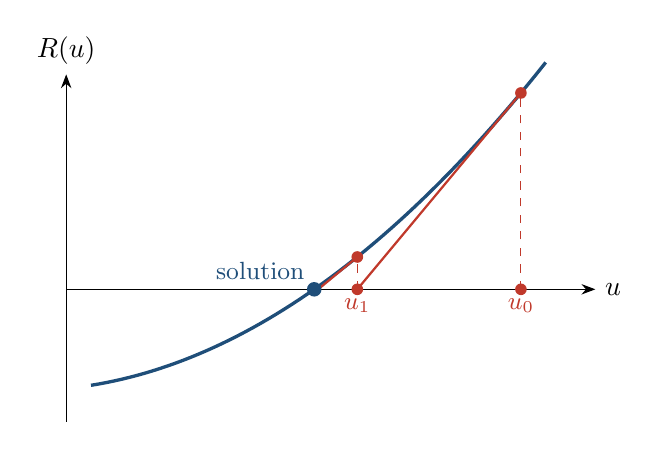
\begin{tikzpicture}[scale=1.05]
  \draw[-{Stealth[length=5pt]}] (0,0)--(6.4,0) node[right]{$u$};
  \draw[-{Stealth[length=5pt]}] (0,-1.6)--(0,2.6) node[above]{$R(u)$};
  % R(u) = 0.1u^2 + 0.1u - 1.2, root u = 3; Newton from u0 = 5.5 gives u1 = 3.52
  \draw[very thick,note,domain=0.3:5.8,samples=60] plot (\x,{0.1*\x*\x+0.1*\x-1.2});
  \draw[dashed,warn] (5.5,0)--(5.5,2.375);
  \fill[warn] (5.5,0) circle (2pt) node[below,font=\small]{$u_0$};
  \fill[warn] (5.5,2.375) circle (2pt);
  \draw[warn,thick] (5.5,2.375)--(3.521,0);
  \draw[dashed,warn] (3.521,0)--(3.521,0.391);
  \fill[warn] (3.521,0) circle (2pt) node[below,font=\small]{$u_1$};
  \fill[warn] (3.521,0.391) circle (2pt);
  \draw[warn,thick] (3.521,0.391)--(3.0476,0);
  \fill[note] (3.0,0) circle (2.5pt) node[above left,font=\small]{solution};
\end{tikzpicture}
\caption{One Newton step: follow the tangent from the current guess to where it
crosses zero. Repeating from $u_1$ converges quadratically.}
\end{figure}

\paragraph{Automatic differentiation: no hand-derived stiffness.}
Deriving $\K$ by hand for a mixed, hyperelastic, follower-load element is long and
error-prone. We avoid it entirely. We only write the \emph{energy} of one element as
a Python function of its 81 nodal coordinates and 4 pressure coefficients, and the
\texttt{jax} library differentiates that function exactly (not by finite
differences):
\begin{itemize}[nosep]
\item \code{jax.grad(_elem_pi)} gives the element force vector (85 entries);
\item \code{jax.hessian(_elem_pi)} gives the element stiffness matrix ($85\times85$);
\item \code{jax.vmap} applies them to all 588 elements at once, and \code{jax.jit}
compiles them to fast machine code the first time they are called.
\end{itemize}
The same is done for the cavity volume and the sleeve energy.

\paragraph{Assembly and the linear solve.}
The condensed element matrices (\eqref{eq:condense}) are added into one sparse global
matrix of size $17\,725\times17\,725$. Its sparsity pattern never changes, so the
index bookkeeping is done once. The linear system is solved with a sparse direct
LU factorisation (SuperLU).

\paragraph{When is it converged?}
A step is accepted when all three hold:
\begin{enumerate}[nosep]
\item the relative force imbalance $\|\R\|/\|\mathbf{f}\|<10^{-9}$;
\item the incompressibility constraint $J-1=p/\kappa$ is met to $10^{-9}$ in every element;
\item under volume control (\S\ref{sec:steps}), the cavity volume matches its target.
\end{enumerate}
The iteration gives up after 15 iterations, if a result becomes NaN, or if the
residual has not halved over the last four iterations.

\paragraph{Safeguard: do not turn elements inside out.}
A full Newton step can be too long and push an element to $J\le0$ (turned inside
out), where $J^{-2/3}$ is undefined and the forces become NaN. The code then halves
the step, $\alpha=1,\tfrac12,\tfrac14,\dots$, until the forces are finite again. This
is a simple \emph{line search}.

\begin{incode}
\code{FEModel.solve} (line 309) is the Newton loop. The \code{jax} derivatives are set
up in lines 268--273; \code{_Assembler} (line 211) does the assembly; \code{spla.splu}
(line 341) factorises; the convergence test is line 326; the step-halving line search
is lines 353--361.
\end{incode}

\begin{pitfall}[Why 64-bit numbers]
\texttt{jax} uses 32-bit floats by default, which are not accurate enough for a
residual tolerance of $10^{-9}$. Line 36 switches on 64-bit arithmetic. Do not remove
it.
\end{pitfall}

%======================================================================
\section{Load stepping and the ballooning limit}
\label{sec:steps}

\paragraph{Why steps.}
Newton's method only converges from a guess close to the answer. Jumping straight
from $P=0$ to $P=100$\,kPa would fail, so the pressure is raised in steps (22 steps
of 5\,kPa for the runs in the deck) and each converged state is the starting guess
for the next.

\paragraph{A better starting guess.}
Instead of starting the next step from the last state, the code extrapolates along
the straight line through the last two states (a \emph{secant predictor}). This
usually saves one or two Newton iterations per step.

\paragraph{Cutting the step.}
If a step fails, it is halved and retried, up to twice. A step is also rejected if
the cavity volume jumps by more than $0.25V_0$, which would mean Newton has leapt to
a distant, snapped-through shape instead of following the path.

\paragraph{The limit point.}
For the bare actuator the pressure--volume curve rises, flattens and reaches a peak
at $P\approx104.7$\,kPa (Figure~\ref{fig:limit}). Beyond the peak there is
\emph{no} equilibrium at a higher pressure: in a real test the thin wall would
balloon suddenly. At the peak the tangent matrix becomes singular, and pressure
steps can no longer converge.

\begin{figure}[H]
\centering
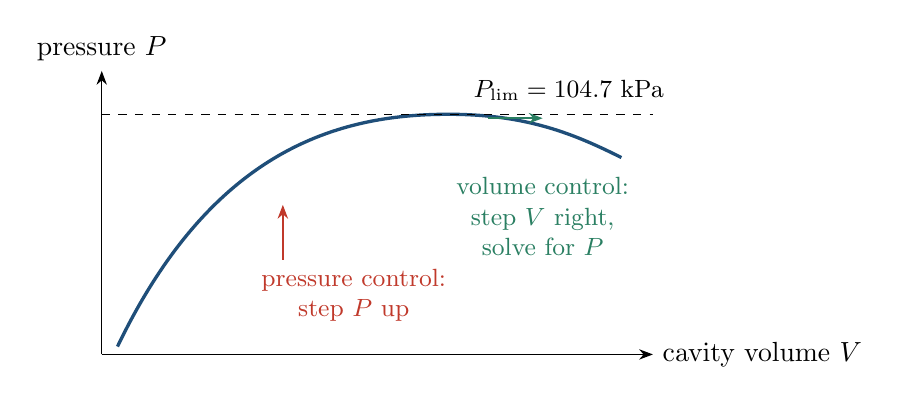
\begin{tikzpicture}[scale=1.0]
  \draw[-{Stealth[length=5pt]}] (0,0)--(7,0) node[right]{cavity volume $V$};
  \draw[-{Stealth[length=5pt]}] (0,0)--(0,3.6) node[above]{pressure $P$};
  \draw[very thick,note] (0.2,0.1) .. controls (1.4,2.6) and (3.0,3.05) .. (4.4,3.05)
     .. controls (5.4,3.05) and (6.0,2.8) .. (6.6,2.5);
  \draw[dashed] (0,3.05)--(7,3.05);
  \node[font=\small,anchor=west] at (4.6,3.35) {$P_{\lim}=104.7$ kPa};
  \draw[-{Stealth[length=5pt]},thick,warn] (2.3,1.2)--(2.3,1.9);
  \node[warn,font=\small,align=center] at (3.2,0.75) {pressure control:\\step $P$ up};
  \draw[-{Stealth[length=5pt]},thick,code] (4.9,3.0)--(5.6,3.0);
  \node[code,font=\small,align=center] at (5.6,1.75) {volume control:\\step $V$ right,\\solve for $P$};
\end{tikzpicture}
\caption{Pressure control cannot pass the peak of the $P$--$V$ curve; volume control
can. The real curve from the FE run is in Figure~\ref{fig:limitreal}.}
\label{fig:limit}
\end{figure}

\paragraph{Volume control.}
The cure is to swap roles: prescribe the cavity volume (as a syringe would) and let
the pressure be the unknown. One extra equation, $V(\uu)=V_{\text{target}}$, is added.
Linearising both equations,
\begin{equation}
\K\,\Delta\uu-\mathbf{g}\,\Delta P=-\R,\qquad \mathbf{g}^{\mathsf T}\Delta\uu=-(V-V_{\text{target}}),
\end{equation}
with $\mathbf{g}=\partial V/\partial\uu$. Solving the first for
$\Delta\uu=\Delta\uu_R+\Delta P\,\mathbf{b}$, with $\K\Delta\uu_R=-\R$ and
$\K\mathbf{b}=\mathbf{g}$, and inserting into the second gives
\begin{equation}
\Delta P=-\frac{(V-V_{\text{target}})+\mathbf{g}^{\mathsf T}\Delta\uu_R}{\mathbf{g}^{\mathsf T}\mathbf{b}} .
\end{equation}
Both solves reuse the same LU factorisation, so volume control costs almost nothing
extra. This ``bordered'' system stays solvable at the peak, so the path can be
followed over the top and the peak pressure read off as the limit pressure.

\paragraph{Switching rule.}
The code ramps under pressure control. When a pressure step still fails after two
halvings, it switches to volume control with volume steps of $0.02V_0$, enlarged by
1.5 after easy steps (at most $0.1V_0$) and halved after failures. It stops when the
pressure starts to fall (the peak has been passed), when the last requested pressure
is reached, or when the volume exceeds $6V_0$.

\begin{figure}[H]
\centering
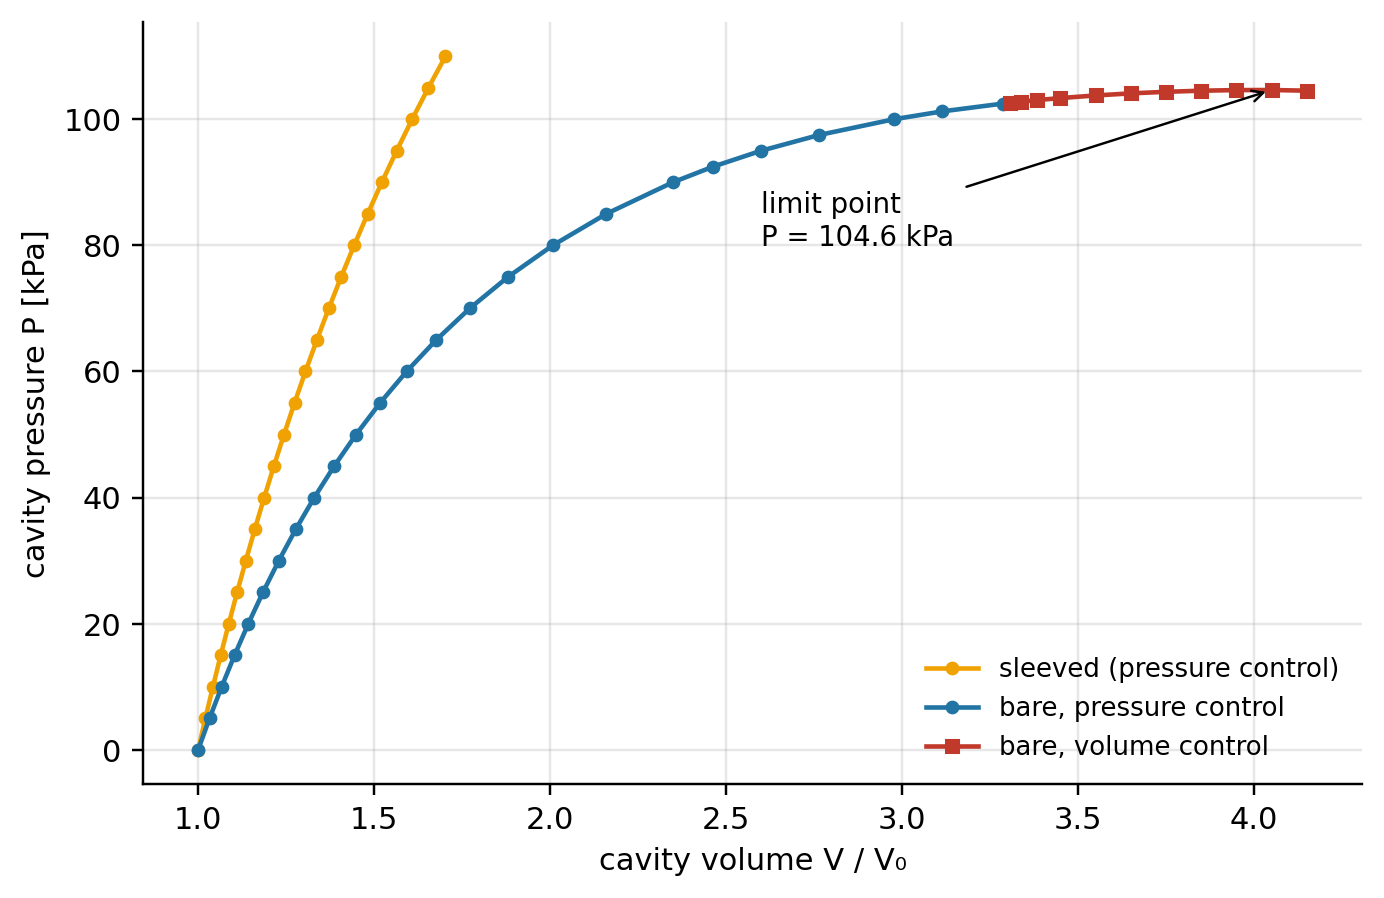
\includegraphics[width=0.72\textwidth]{figures/fe_limit_point.png}
\caption{The FE pressure--volume path. The sleeved actuator (orange) stays on the
rising branch; the bare actuator (blue) reaches its limit and is followed past it
under volume control (red).}
\label{fig:limitreal}
\end{figure}

\begin{incode}
\code{simulate} (line 399): the \code{predictor} (line 414), the pressure loop with
step halving (lines 426--447) and the snap-through check (line 434), the
volume-control loop (lines 449--463), and the limit pressure \code{P_limit} (line
472). The bordered solve is lines 344--348 of \code{FEModel.solve}.
\end{incode}

%======================================================================
\section{Post-processing: from displacements to tip deflection}
\label{sec:post}

The solver returns the displacement of every node. The quantities we report are
extracted from two lines of nodes on the symmetry plane: the top line of the outer
surface ($y=+R$, thin side) and the bottom line ($y=-R$, thick side).
\begin{itemize}[nosep]
\item At each $x$, the vector from the bottom to the top node gives the rotation of
the cross-section, $\theta=\operatorname{atan2}(d_x,d_y)$; its midpoint is the beam
axis.
\item The \textbf{tip angle} and \textbf{tip deflection} are $\theta$ and $\delta=-c_y$ at
$x=L$, the end of the pressurised length (positive towards the thick wall).
\item The \textbf{curvature} is the slope of $\theta$ against $x$ over the middle half
of the actuator, away from the clamp and the cap.
\item Also recorded: axial stretch of the axis, diameter and cavity stretch at
mid-span, thin-wall thickness relative to its original 3\,mm, cavity volume and the
largest principal stretch.
\end{itemize}

\begin{incode}
\code{measure} (line 370). \code{save} (line 479) writes \texttt{summary.csv} (one row
per pressure), \texttt{results.npz} (all fields) and \texttt{run.json} (inputs);
\texttt{fea\_viewer.py} turns them into an interactive \texttt{viewer.html}.
\end{incode}

%======================================================================
\section{Checking the code: verification}
\label{sec:verify}

A new FE code must be tested on problems whose answers are known before its
predictions are trusted. \texttt{fea\_verify.py} runs four such tests
(Figure~\ref{fig:verify}).

\begin{center}
\begin{tabularx}{\textwidth}{@{}l X r@{}}
\toprule
Test & What it checks & Worst error\\
\midrule
1 Uniaxial tension & material law and large stretch; exact stress formula, $\lambda$ up to 3
 & 0.2\,\% (neo-Hookean)\\
2 Thick-tube inflation & follower pressure, volume formula; exact neo-Hookean solution
 & 0.05\,\%\\
3 Small-pressure bending & the $(1-2\nu)$ law of the derivation report, $\nu$ from 0 to 0.4995
 & 0.0002\\
4 Mesh convergence & medium vs fine mesh, tip deflection at $P/\mu=0.30$ and $0.45$
 & 0.5\,\%\\
\bottomrule
\end{tabularx}
\end{center}

The Yeoh case in test 1 differs by up to 2.5\,\% at $\lambda=3$. That is expected,
not a bug: the exact formula assumes perfect incompressibility, while the code uses
a finite $\kappa$ ($\nu=0.4995$), and the difference grows with the stiffening Yeoh
terms at large stretch.

\begin{figure}[H]
\centering
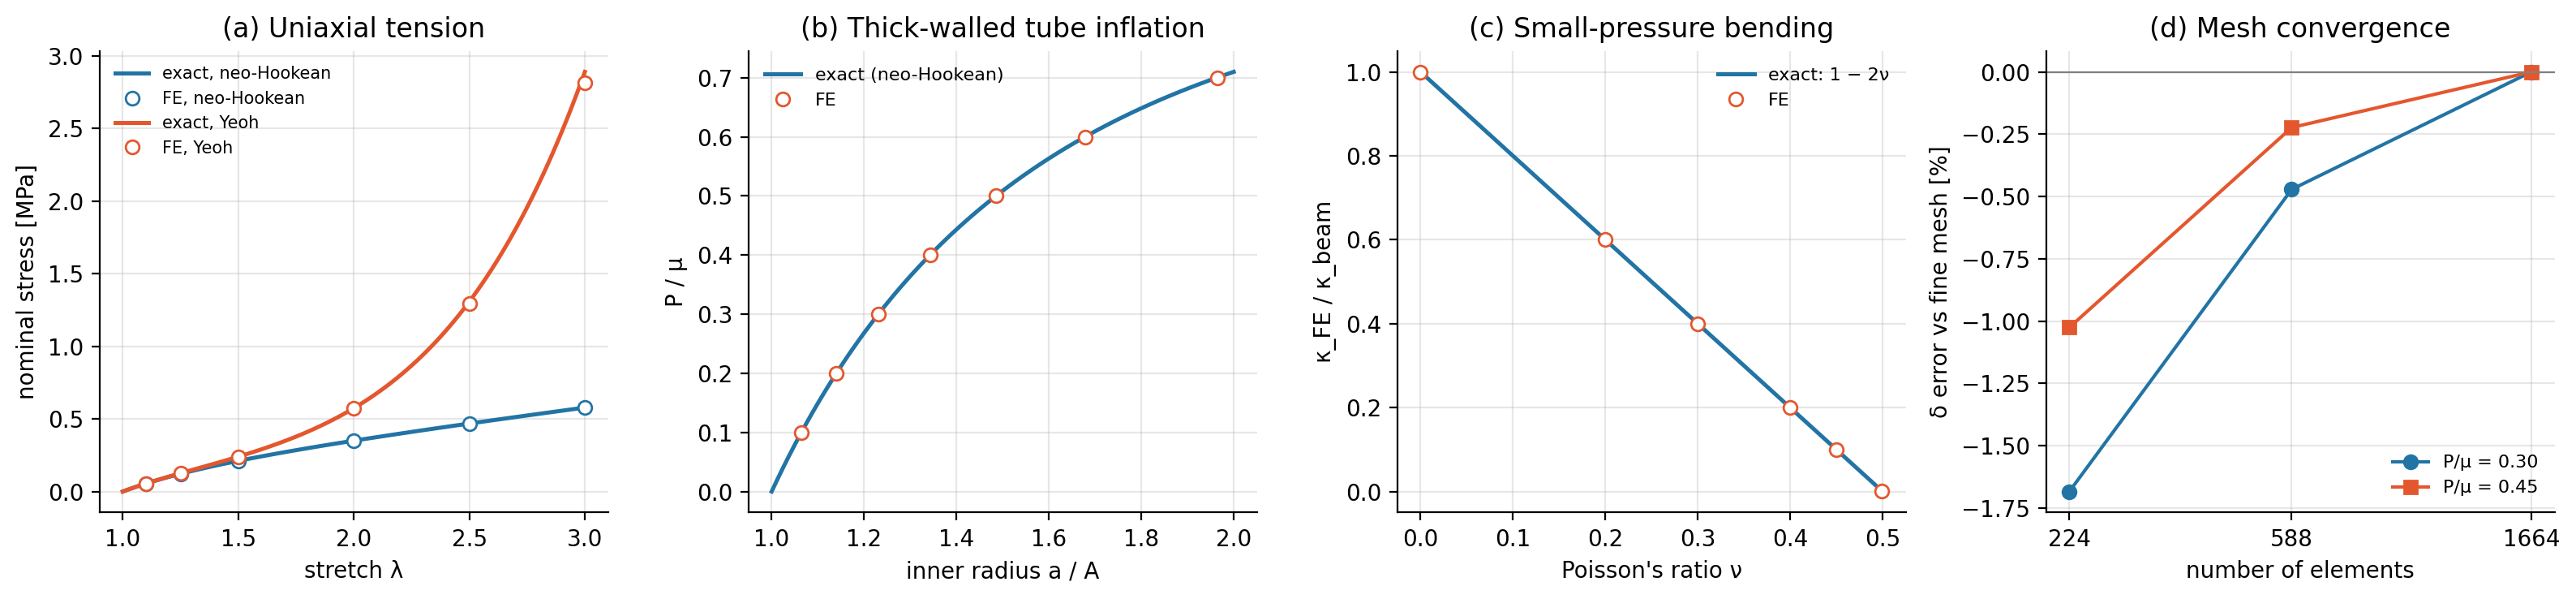
\includegraphics[width=\textwidth]{figures/fe_verification.png}
\caption{The four verification tests (from \texttt{results/verification.log}).}
\label{fig:verify}
\end{figure}

%======================================================================
\section{What the runs give}
\label{sec:results}

Two pressure sweeps were run on the medium mesh with the placeholder geometry and
silicone: the bare actuator (36 converged states, 177\,s) and the sleeved actuator to
110\,kPa (23 states, 103\,s). The full discussion is in the derivation report and the
slides. In short:
\begin{itemize}[nosep]
\item the bare actuator barely bends at low pressure ($\delta$ grows as $P^2$), then
balloons and reaches its limit at 104.7\,kPa;
\item the sleeved actuator bends smoothly and nearly linearly, 16.3\,mm at 60\,kPa
against 5.9\,mm for the bare one;
\item the beam models of the derivation track the sleeved FE within 5\,\% at low
pressure and fall 20--25\,\% short by 60\,kPa.
\end{itemize}

\begin{figure}[H]
\centering
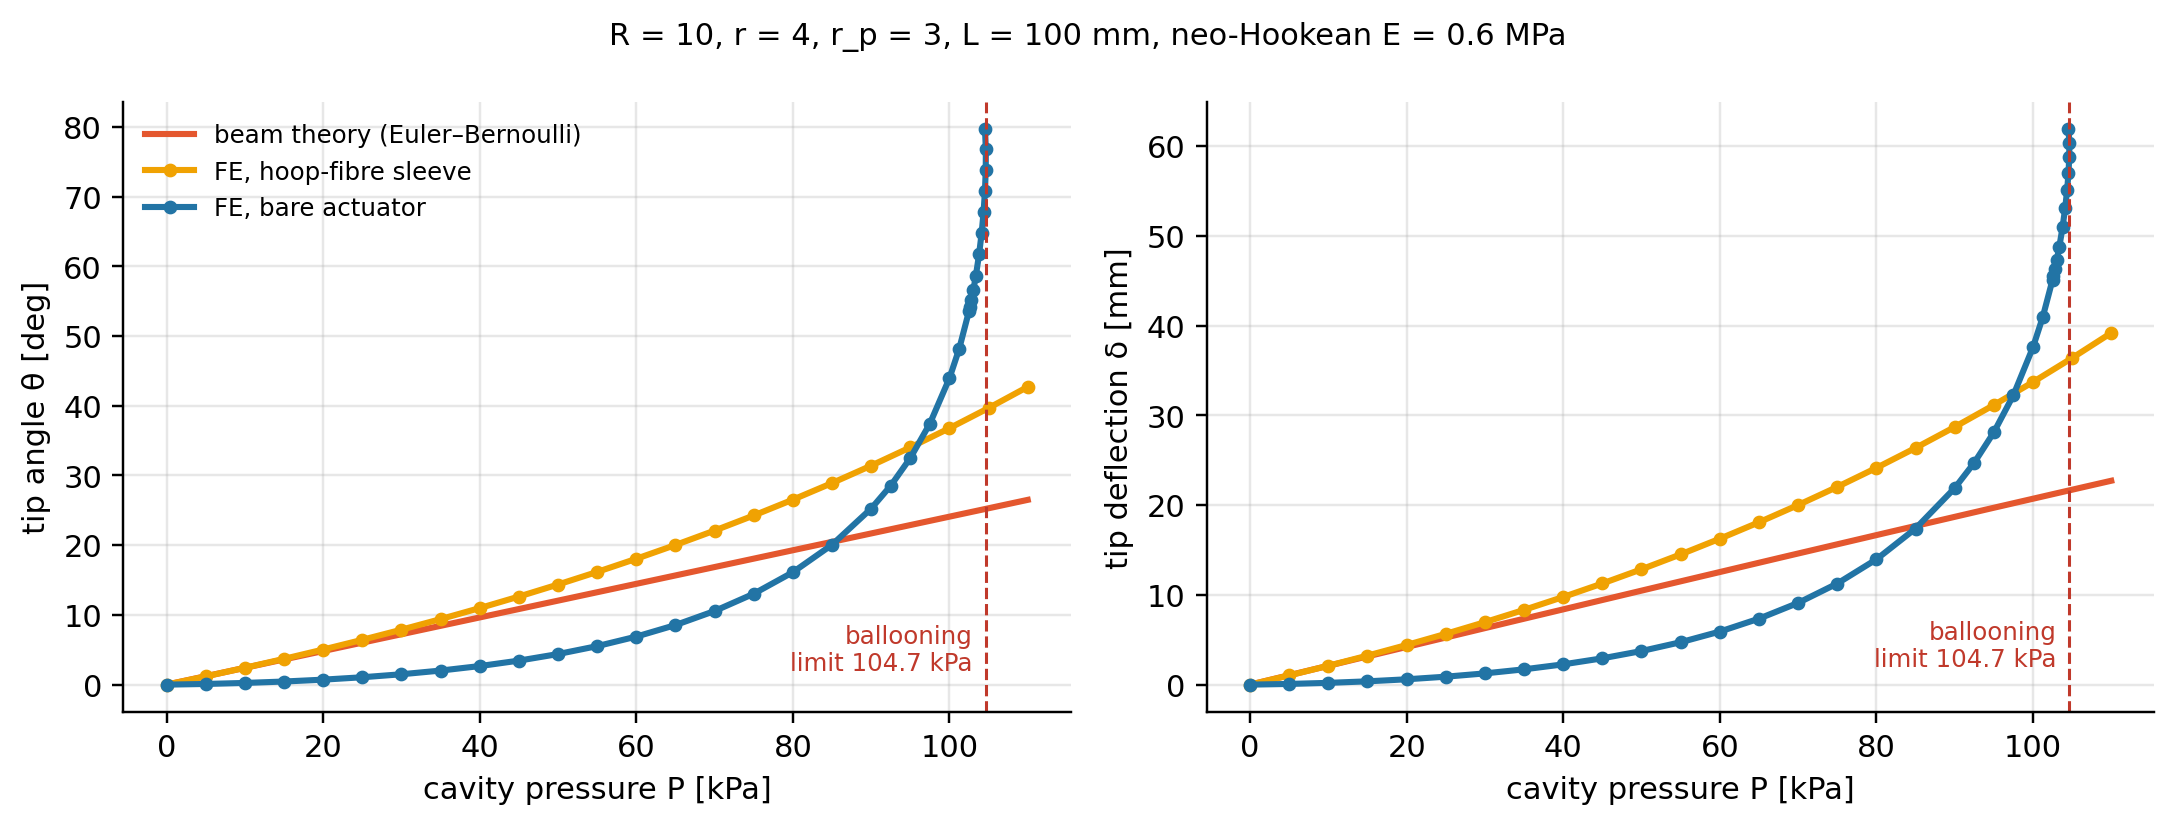
\includegraphics[width=\textwidth]{figures/fe_response.png}
\caption{Tip angle and tip deflection against pressure: beam theory, bare and
sleeved FE.}
\end{figure}

\begin{figure}[H]
\centering
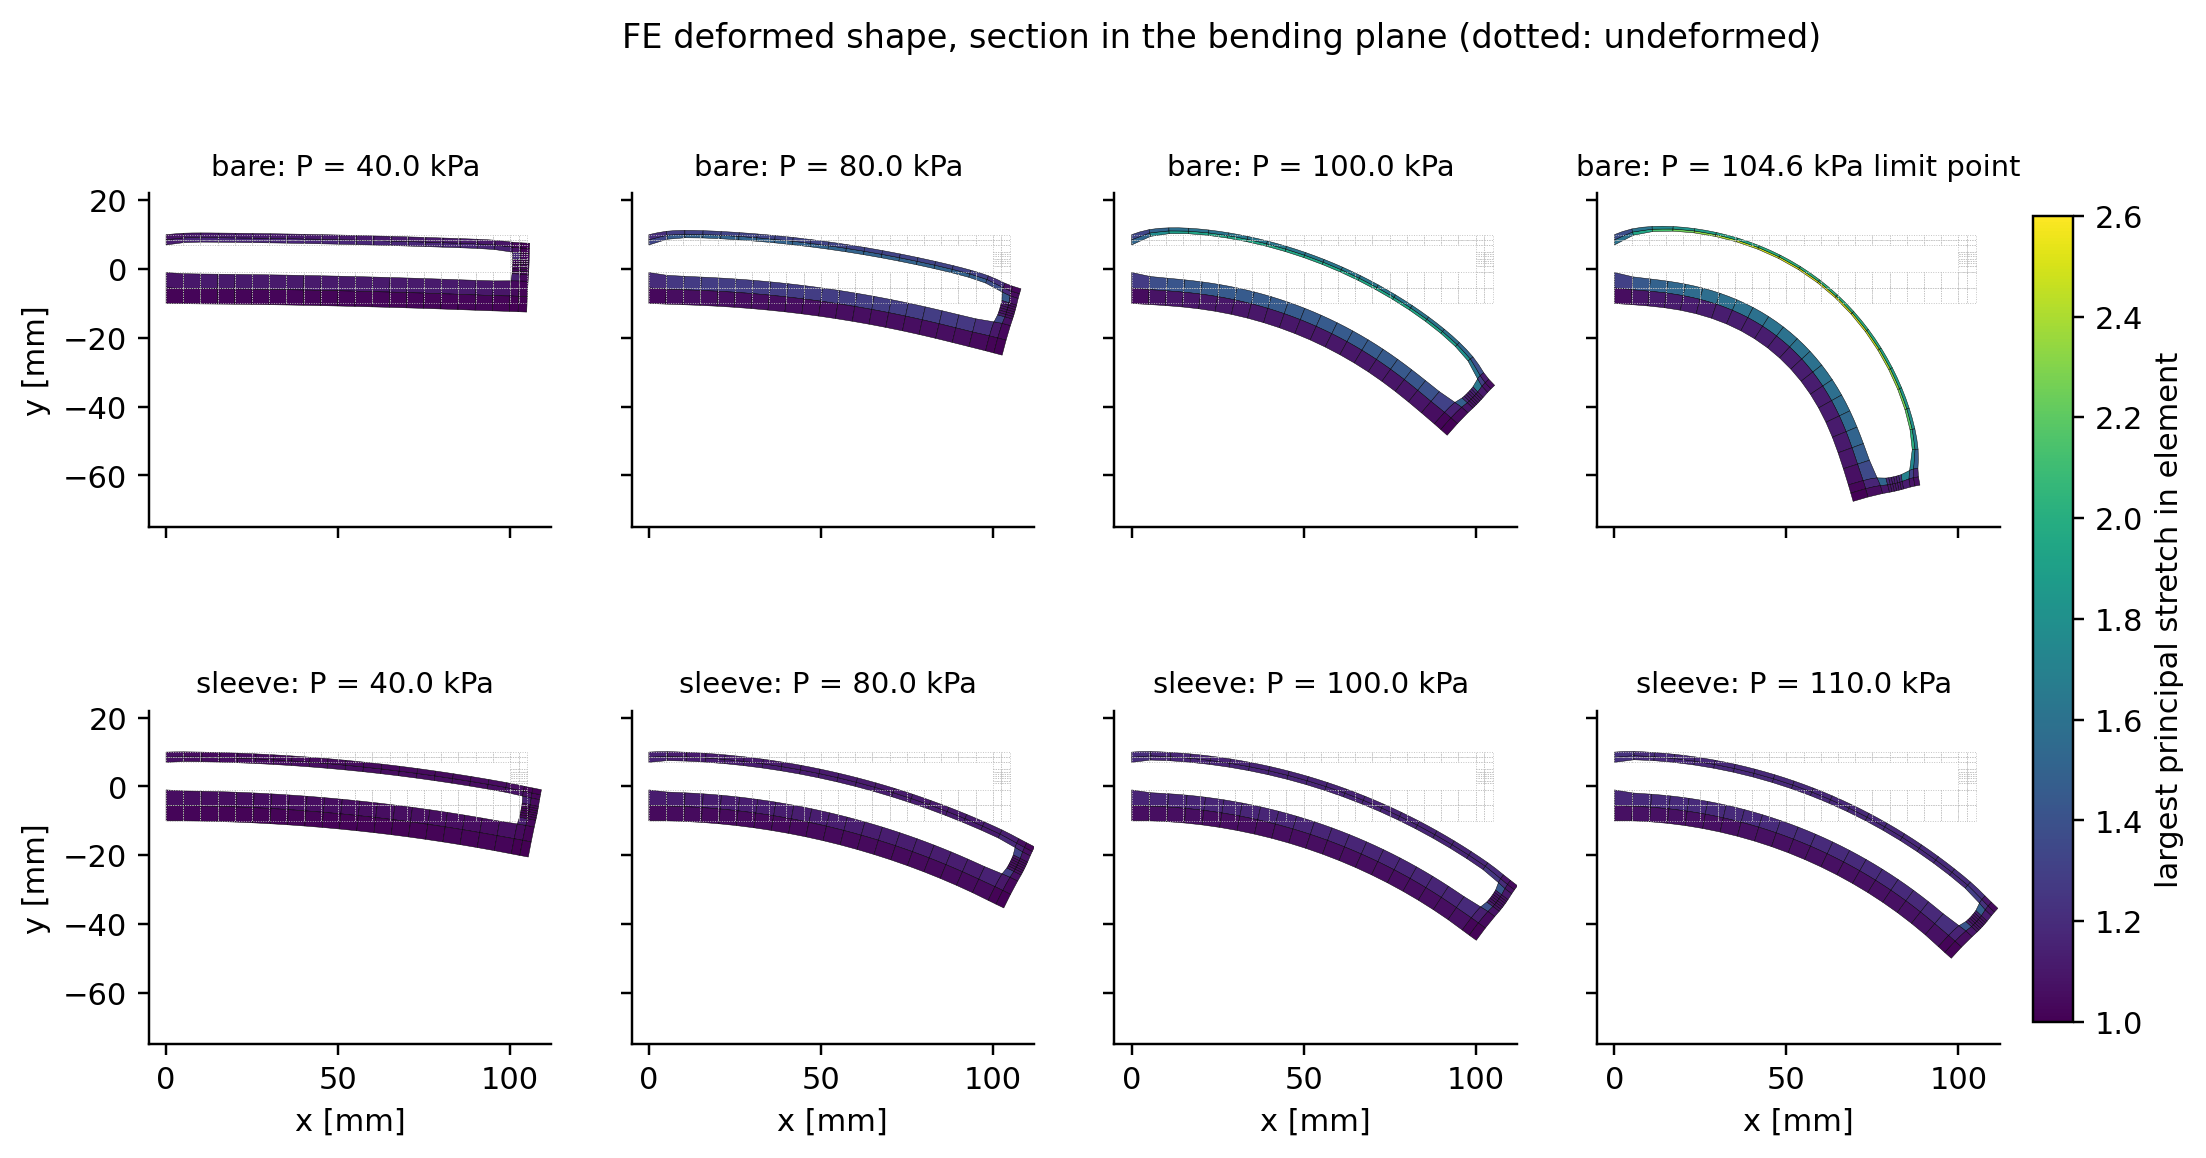
\includegraphics[width=\textwidth]{figures/fe_deformed_sections.png}
\caption{Deformed bending-plane sections, coloured by the largest principal
stretch.}
\end{figure}

%======================================================================
\section{Running and changing the code}
\label{sec:run}

\paragraph{A pressure sweep.}
From the project folder:
\begin{lstlisting}[language=bash]
python actuator_fea.py --R 10 --r 4 --rp 3 --L 100 --E 0.6 --pmax 110 --steps 22 --out results/bare
python actuator_fea.py --R 10 --r 4 --rp 3 --L 100 --E 0.6 --pmax 110 --steps 22 --sleeve --out results/sleeve
python -u fea_verify.py
python fea_compare.py results/bare results/sleeve
\end{lstlisting}
Each sweep prints one line per converged state (pressure, volume ratio, tip
deflection, Newton iterations, elapsed time) and ends by writing
\texttt{summary.csv} and an interactive \texttt{viewer.html}.

\paragraph{What to change, and where.}
\begin{center}
\begin{tabularx}{\textwidth}{@{}l X@{}}
\toprule
To change & Do this\\
\midrule
geometry & \opt{R} \opt{r} \opt{rp} \opt{L}, and \opt{tcap} for the tip cap\\
silicone (measured) & \opt{yeoh C10 C20 C30} from the tensile-test fit\\
reinforcement & add \opt{sleeve}\\
pressure range & \opt{pmax} (kPa) and \opt{steps}\\
accuracy vs speed & \opt{mesh coarse}, \code{medium} or \code{fine}\\
compressibility & \opt{nu} (keep it at 0.4995 for silicone)\\
\bottomrule
\end{tabularx}
\end{center}

\section{Troubleshooting}
\label{sec:trouble}

\begin{description}[style=nextline,leftmargin=0.6cm,font=\normalfont\bfseries]
\item[``inverted element in the mesh''] The geometry is invalid, usually $r+r_p\ge R$
(the cavity cuts through the outer wall). Check the inputs.
\item[A pressure step fails repeatedly] Use more steps (smaller $\Delta P$). If it
happens near the top of the range on a bare actuator, it is the ballooning limit, and
the switch to volume control is the correct behaviour.
\item[The run is slow] The first call compiles the \texttt{jax} functions (tens of
seconds). After that a medium sweep takes 2--3 minutes on a laptop. The fine mesh
takes roughly five times longer.
\item[Results look too stiff] Check that $\nu$ was not set much closer to 0.5 and
that the mixed formulation was not removed; both would bring back locking.
\item[Long runs vanish] Write the log to a file with \code{python -u ... > run.log}
and watch the file; very long background jobs may be stopped by the terminal.
\end{description}

%======================================================================
\appendix
\section{Code map}

\begin{center}
\small
\begin{tabularx}{\textwidth}{@{}l r X@{}}
\toprule
Name in \texttt{actuator\_fea.py} & Line & What it does\\
\midrule
\code{_lagrange}, \code{_GP}, \code{_GW} & 41--50 & 1-D quadratic shape functions, Gauss points and weights\\
\code{_tp3}, \code{DN3}, \code{W3}, \code{PSI} & 54--59 & 27-node brick: derivatives, weights, pressure basis\\
\code{MESH_PRESETS} & 68 & coarse / medium / fine mesh sizes\\
\code{merge_blocks} & 87 & glue mesh blocks, number nodes along $x$\\
\code{right_handed}, \code{orient_faces} & 106, 114 & fix element and face orientation\\
\code{build_mesh} & 131 & half-actuator mesh from rays $\rho_{\text{out}}(\phi)$ and the cap\\
\code{_elem_pi} & 184 & mixed Yeoh energy of one element\\
\code{_face_volume} & 194 & cavity volume from one face\\
\code{_sleeve_energy} & 203 & hoop-fibre energy of one outer face\\
\code{_Assembler} & 211 & sparse global matrix with a fixed pattern\\
\code{FEModel.__init__} & 245 & $\kappa$, $\mathbf{A}$, \code{dNdX}, \code{jax} derivatives, free unknowns\\
\code{FEModel.forces} & 292 & internal forces, $\partial V/\partial\uu$, constraint residuals\\
\code{FEModel.stretch} & 303 & largest principal stretch per element\\
\code{FEModel.solve} & 309 & Newton loop, condensation, volume control, line search\\
\code{measure} & 370 & tip angle, deflection, curvature, stretches, wall thickness\\
\code{make_actuator} & 388 & mesh, clamp, symmetry, sleeve stiffness\\
\code{simulate} & 399 & pressure ramp, step cutting, switch to volume control\\
\code{save} & 479 & write \texttt{results.npz}, \texttt{summary.csv}, \texttt{run.json}\\
command line & 506 & options and defaults\\
\bottomrule
\end{tabularx}
\end{center}

\section{Glossary}

\begin{description}[leftmargin=0.6cm,font=\normalfont\bfseries,itemsep=2pt]
\item[Assembly] Adding each element's small matrix into the right rows and columns of the global matrix.
\item[Automatic differentiation] Computing exact derivatives of a program by applying the chain rule to every operation (here, \texttt{jax}).
\item[Deformation gradient $\F$] The matrix that maps small fibres from the undeformed to the deformed body.
\item[Follower load] A load whose direction follows the deforming surface, such as gas pressure.
\item[Gauss point] A point inside an element where the integrand is evaluated for numerical integration.
\item[Hyperelastic] A material whose stress follows from a stored-energy function $W$.
\item[Isoparametric] Using the same shape functions for the geometry and the displacement.
\item[Limit point] A peak of the load--response curve; beyond it the load cannot increase.
\item[Locking] Artificial over-stiffness of displacement-only elements for nearly incompressible materials.
\item[Mixed (u--p) element] An element with displacement and pressure unknowns, which avoids locking.
\item[Newton--Raphson] Iteration that repeatedly solves the linearised equations; converges quadratically near the solution.
\item[Residual] The out-of-balance nodal force; zero at equilibrium.
\item[Shape function] The interpolation function attached to one node of an element.
\item[Static condensation] Eliminating element-internal unknowns before assembly.
\item[Tangent stiffness] The derivative of the residual with respect to the displacements.
\item[Volume control] Prescribing the cavity volume and solving for the pressure, used to pass a limit point.
\end{description}

\end{document}
